\documentclass[annual]{styles/acmsiggraph}
\usepackage{graphicx}
\usepackage{pdfpages}
\title{A Comparison between Linear Blend Skinning and Dual Quaternion Skinning}
\author{Abdulaziz Almaslukh\thanks{e-mail:almasluk@usc.edu}\\
\and Gautham Shankar Ravishankar\thanks{e-mail:gravisha@usc.edu}\\
\and Karthik Srinivasan\thanks{e-mail:srinivak@usc.edu}\\
\and Nasser Alrayes\thanks{e-mail:alrayes@usc.edu}\\
\and \\
Computer Science Department,\\
Viterbi School of Engineering,\\
University of Southern California.}
\pdfauthor{Karthik Srinivasan}

\keywords{Character Animation, Skinning, Linear Blend, Dual Quaternion, Geometric Deformation, Modelling}

\begin{document}
 \teaser{
 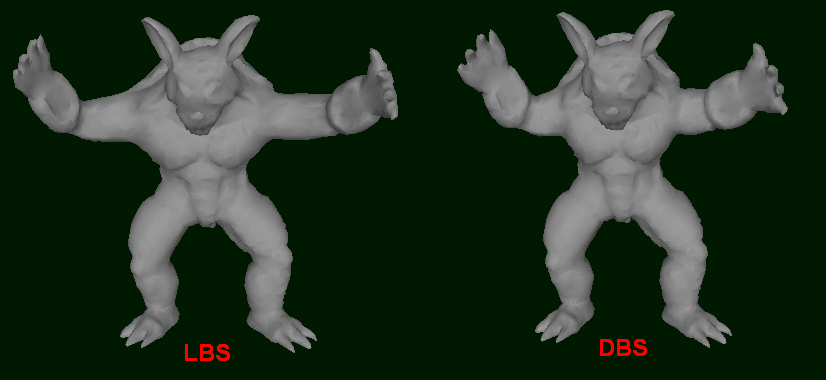
\includegraphics[height=1.5in]{images/teaser}
 \caption{Comparison between Linear Blend Skinning &(LBS&) and Dual Quaternion Blend Skinning &(DBS&)}
 }
\maketitle
\begin{abstract}
In character animation, the basic challenge is to modify the geometry of a given model depending upon the movement of the character. For instance, when a character opens its arms wide open then the polygon meshes in the chest area of the character has to expand. It's similar to how human muscles change shape with respect to the motions. The most widely used technique to tackle this challenge is Linear Blend Skinning &(LBS&) ~\cite{Jacka:2007:CLS:1294685.1294715}. However, they have well documented artifacts which requires an artist to intervene the process to rectify the artifacts. In this paper, we try to explain why LBS is widely used and decribe their artifacts by implementing it. Further, Dual Quaternion Blend Skinning~\cite{Kavan-07-SDQ} is studied, implemented and compared with LBS as an alternative approach.
\end{abstract}
\keywordlist
\section{Introduction}

Character animation is the process of moving the character in a life like manner. Similar to how living beings control their movements by controlling the joints of their bone, in character animation, a skeleton structure is embedded into the character model. The process of binding the skeleton with the character is known as \textit{Character Rigging}. Then, the character is animated by moving the skeleton bones. During the animation, the triangles that form the character model has to move and deform along with the skeleton. The process of deforming and moving triangle mesh based on the movements skeleton is known as \textit{Character Skinning}. There are several approaches to skinning with varying degrees of realism and complexity such as Linear Blend Skinning, Log Matrix Blend Skinning, Spherical Blend Skinning and so on.

In this paper, we are comparing two different skinning methods: the Linear Blend Skinning &(LBS&) and the Dual Quaternion Skinning &(DBS&)~\cite{Kavan-07-SDQ}. Linear Blend Skinning is known for its simplicity and efficiency. As a result, linear blend skinning is still the number one choice for the majority of developers. The basic principle is that skinning transformations are represented by matrices and blended linearly. It is very well known that the direct linear combination of matrices is a troublesome way of blending transformations. Therefore, this technique produces artifacts in the deformed skin such as elbow collapse, even if we restrict the skinning transformations to rigid ones &(i.e., composition of a rotation and translation&). We show that Dual Quaternion Skinning approach solves the artifacts of linear blend skinning at minimal additional cost. Upgrading an existing animation system (e.g., in a videogame) from linear to dual quaternion skinning is very easy and has negligible impact on run-time performance. The rest of the paper is organized as follows: In the following section, we will discuss about the system design and decision and the input it requires. In section (III) we will talk about Linear Blend Skinning and how it is implemented, then we will discuss Dual Quaternion Skinning as a solution for LBS artifacts in section (IV). In section (V) we will show our comparison results between LBS and DQS. Finally, in section (VI) we talk about our conclusions for this paper.  

\section{Overview}

The intial criteria for the animation system was to develop it over the homework system that we used in CSCI 580 course at USC. The reason for establishing this criteria was because of the varying level of knowledge between us and we thought that building the system over the homework system would help us in colloborating efficiety. Hence, the initial processing of input files and the implementation of the techniques was done as an extension to homework system. However due to the inflexbility of the homework system, we had to develop a new system based on OpenGL to support character animation. We will discuss about the input data briefly in the below section.

\subsection{Character Animation Input Files}

In Character Animation, there are various type of numerical data that are fed into the animation system to acheive the desirable results. These numerical data determine the character features, the environment, the interaction of the character with the environment, the texture and so on. Since, our primary goal is to study the character skinning techniques, we would consider the least required set of numerical data for character animation:

\begin{enumerate}
\begin{figure}[ht]
  \centering
  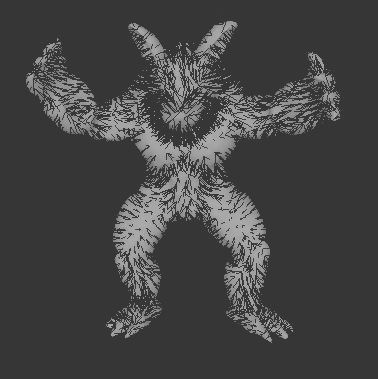
\includegraphics[width=2in]{images/normals}
  \caption{Character model highlighting the Vertex Normals}
  \label{normals}
\end{figure}

\item The model file for the character consists of data for triangle meshes. In this project we tried working with different models that was freely available on the internet. A typical character model can consist of anywhere between 10,000 and 100,000 triangles. Hence, it’s very important to load and process the data into an easily accessible data structure at the beginning of the animation, to reduce the latency and improve frame rate while creating animation. The input files we used, follows a format where the vertex data is listed down separately and then each triangle is mapped to vertex by using vertex number. The input files did not contain the normals of each vertex that is needed for rendering, hence we calculated the normals at each vertex by tracking adjacent triangles of each vertex and its normals. The figure~\ref{normals} hightlights the normals at each vertex that was computed. Later, we came to know that there are open source library function which computes the normals at each vertex.

\begin{figure}[ht]
  \centering
  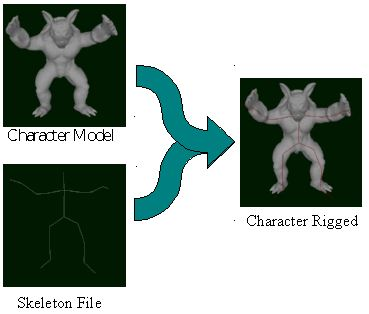
\includegraphics[width=2.2in]{images/rigg}
  \caption{Illustration of Character Rigging.}
\end{figure}

\item The skeleton data file, which enables us to control the character. The process of generating and embedding the skeleton for a given character model is called character rigging. The complexity of the character animation is determined by the complexity of the skeleton structure and number of bones in it. In this project, we used a simple 21 bone skeleton structure that was generated using an automatic character rigging library, Pinocchio~\cite{Baran:2007:ARA:1275808.1276467}. 
\begin{figure}[ht]
  \centering
  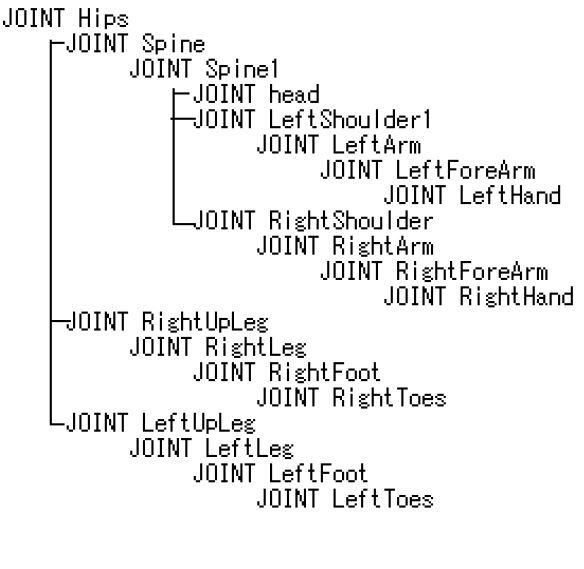
\includegraphics[width=1.8in]{images/ske2}
  \caption{Hierarchical Structure of the Skeleton.}
  \label{hier}
\end{figure}
The skeleton structure is required to be processed to compute relative position of each bone with its parent and origin. Initially, the skeleton is processed listed in the hierarchical structure as shown in the figure~\ref{hier}, where the hip joint is considered as the root joint of the skeleton. The root joint is selected based on the requirement of animation, the widely used root join is usually placed at the groin region of the character because it gives added stability during skinning process when compares to other joints. 
\begin{figure}[ht]
  \centering
  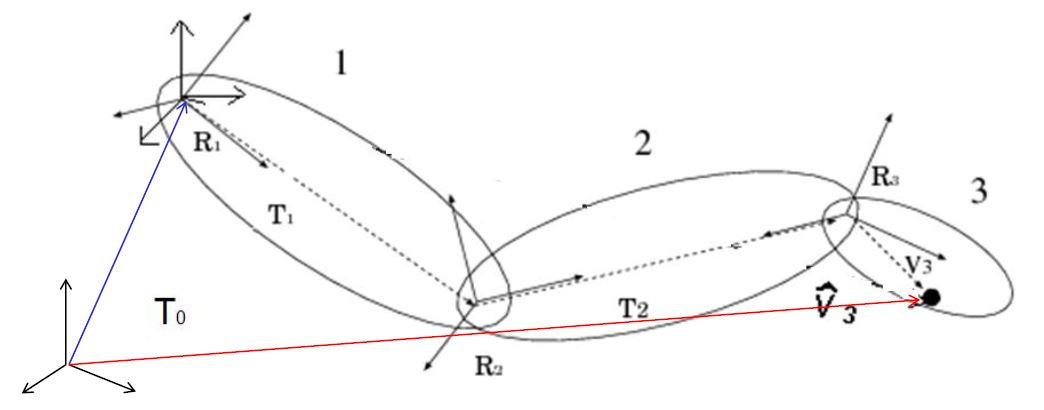
\includegraphics[width=2.1in]{images/skelet}
  \caption{Bone to World transformation of Vertices}
  \label{bw}
\end{figure} \\
After establishing the hierarchy, each bone is assigned with a rotation matrix, R$_{\text{i}}$ and a translation matrix, T$_{\text{i}}$ (i representation the bone indices) which is defined with respect to it’s parent bone, for instances the matrices of right ankle depends on right knee. The rotation matrix for each bone is initialized to identity matrix for the rest pose of the character. The translation matrix is defined based on the length and direction of the bone in rest position. Next, inverse of the rest pose bone matrix, P$_{\text{i}^{\text{-1}}}$ is calculated, which defines each bone with respect to origin of the world. Figure~\ref{bw} shows how the vertex can be defined with respect to the origin of the world.

\[P_{i}^{-1} = (T_{i}R_{i}P_{j})^{-1}\]where i and j represents bone indices and bone j is parent of bone i.
\[V=P_{i}^{-1}\widehat{V}\] where $\widehat{V}$ is vertex in bone space and V is vertex in world space.

\item Set of numerical data which determines the relation between a triangle in the model and a bone in skeleton structure. For example the triangles which forms the arm of the character is binded to the bones that represent the arms. The data is represented using set of floating point values for each vertex which binds it to the bones in skeleton. We considered a 21 bone skeleton structure for our study, therefore each vertex would consist of 21 floating point values which will add up to total of 1.
\[\sum_{i=1}^{n} W_{i}=1\] where i is bone indices and n is total number of bones.
\end{enumerate}

\section{Linear Blend Skinning}
Linear Blend Skinning (LBS), also known as Skeleton Subspace Deformation (SSD) and smooth skinning, is the most popular and widely used method for character deformation and animation. The most important reason to its success is its low computational complexity and it’s easy to implement as \textit{Shader Program} on GPU. LBS determines the new position of a vertex,$\widehat{V}$ with normal $\widehat{V_{\text{N}}}$  by linearly combining the results of the vertex transformed rigidly with each bone. A scalar weight, W$_{\text{i}}$ , is given to each influencing bone and the weighted sum gives the vertex’s new position, V with new normal,V$_\text{N}$ in the new pose, as follows:

\[V= \sum_{i=1}^{n}W_{i}T_{i}R_{i}P_{i}^{-1}\widehat{V}\]
\[V_{N}= \sum_{i=1}^{n}W_{i}T_{i}R_{i}P_{i}^{-1}\widehat{V_{N}}\]

For bones which have no influence on the movement of a vertex, the associated weight would be 0. As mentioned earlier, the sum of all weights is equal to 1.  So basically to transform the character from rest position to new position, the rotation matrix and translation matrix of the bones are changed. and new bone pose position Matrix is calculated for each bone. While transforming the vertex and normals of the triangle mesh, we use this linear weighted formula, which transforms the vertex to the origin and then performs the rotation and then does the translation to take it back to the position with respect to it’s parent bone. This is very similar to the technique we learned in class for implementing solar system.

\begin{figure}[ht]
  \centering
  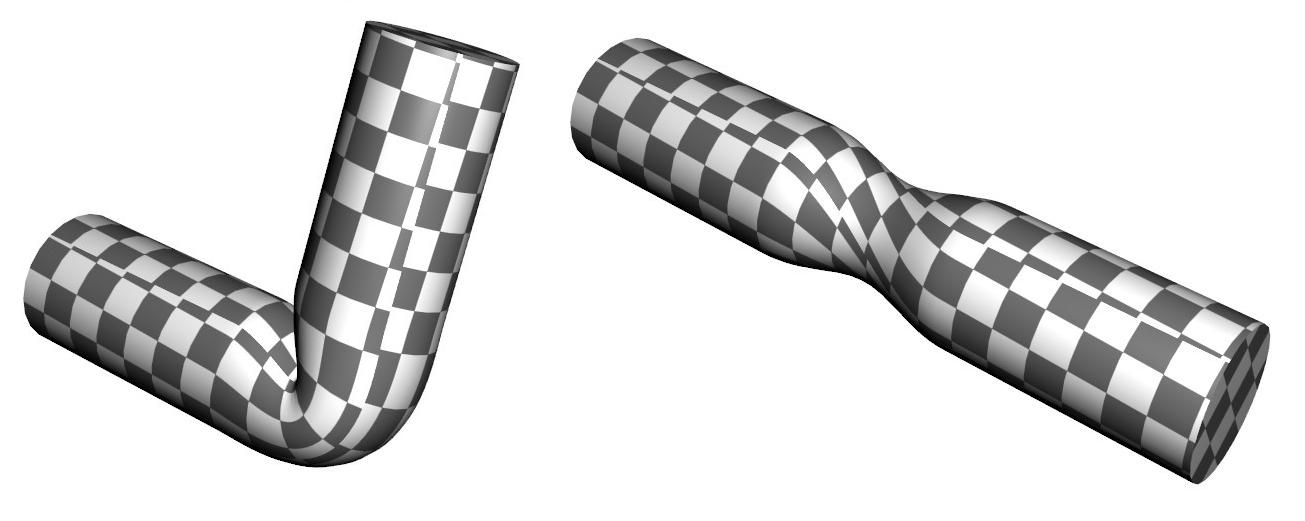
\includegraphics[width=2.1in]{images/candy}
  \caption{Collapsing of joint and \textit{Candy Wrapper} effect.}
  \label{bw}
\end{figure}

However, LBS suffers from few problems such as the elbow collapse and the candy wrapper artifacts (see Fig.1). These problems happen because each skin vertex is assigned multiple influences and blending weights for each joint. This scheme provides more detailed control over the results. However, the generated meshes cause volume loss as joints are rotated to extreme angles producing non-natural deformations (collapsing elbow and candy wrapper effects). Yet another problem with LBS is that tuning the LBS vertex weights tends to be a tedious. Despite these drawbacks, variations of this method are widely used in interactive computer graphics applications because they are simple and easy to implement on GPUs.

\section{Dual Quaternion Skinning}
Dual quaternion skinning is a method of skinning that addresses commonly associated problems with linear blend skinning. By using an approximate blending method, dual quaternion skinning is able to achieve comparable speeds to linear blend skinning, while still retaining the increase in visual quality. This technique utilizes dual numbers to extend quaternions to represent both rotation and translation. This allows for an efficient representation of the transformations and for application of low-cost linear blending.

Dual-quaternions are a combination of dual-number theory and quaternion mathematics. Quaternion and dual-quaternion components are shown in Fig 2. While a quaternion consists of four scalar values, a dual-quaternion consists of eight scalar values. A quaternion is a scalar, vector pair; it consists of a scalar value and a three-dimensional vector value. Dual quaternion is a extended version of quaternion, which consists of two quaternions, namely real and imaginary quaternion. In this representation, the rotational matrix ri of each bone is represented using real part of the dual quaternion and translation ti of each bone is represented using the imaginary part. Typically a pair of rotation and translation data requires 12 variables, 9 for rotation and 3 for translation whereas dual quaternion uses just 8 variables. Thus, Dual quaternions are more memory efficient, requiring only 8 floats per transformation), instead of the 12 required by matrices. However, a quaternion can only represent rotation, while a dual-quaternion can represent both rotation and translation.

In any existing application, it is extremely easy to replace a linear blend skinning implementation by a dual quaternion one. All that is necessary is a slight modification of the vertex shader and conversion of the matrices to dual quaternions before passing them to the shader. The model files as well as the internal data structures do not need any change at all – the only difference is in the transformation blending.
Implementing dual quaternion skinning is straight forward. First, we need to convert the skinning matrices C1, . . . ,Cp (where p is the total number of joints) to dual quaternions ˆq1, . . . ,ˆqp, The next task is to compute a blended unit dual quaternion ˆq with respect to the given convex weights w = (w1, . . . ,wn). This can be done by taking their linear combination followed by a normalization (because we need a unit dual quaternion). We call this Dual quaternion Linear Blending (DLB):

This will typically be done on a CPU and will not take long, because the conversion to a dual quaternion involves just one quaternion multiplication and the number of joints p is usually quite small. The dual quaternions ˆq1, . . . , ˆqp are then sent to the GPU as uniform parameters, each represented by a 2x4 matrix. Dual quaternion skinning can thus be summarized in the following pseudocode:

\section{Results and Comparison}
Instead of relying on additional weights or alternative rigging metaphors we directly solve the joint collapse and candy-wrapper artifacts in LBS by implementing DQS through blending rigid bone transformations as dual quaternions rather than matrices, leaving the skeleton and bone weights metaphor untouched. (see Fig. 3)

In order to bend properly, the bone weights in an LBS or DQS rig must only overlap close to the joints. As a result these methods must pack interesting twisting near joints. LBS linearly blends rotation matrices, resulting in the candy-wrapper effect. DQS corrects this artifact by blending rotations as quaternions. We have applied both methods to our character (see Fig. 4) to evaluate and analyze the collapsing elbow problem. In its twisted state, the arm is bent at the elbow. Joint collapse artifacts are corrected by switching to DQS as the underlying skinning formulation. In contrast, using LBS results in joint collapse, isolated twisting and shape explosion which are prevented by applying DQS.

\section{Conclusion}

We have shown in this paper two different skinning methods which are Linear Blend Skinning and Dual Quaternion and that the later method can solve the artifacts of Linear Blend Skinning such as candy wrapper and elbow collapse. We have shown that the implementation of Dual Quaternion Skinning is simple and efficient and fast to execute and render and Linear Blend Skinning.
In future work, we would like to explore further the different skinning methods and the role they play in character animation.  It would be interesting to expose the artifacts of each of those methods and compare different techniques to solve them and measure their time and space complexity. Moreover, it would be interesting to control advanced effects such as muscle bulging and applying simple filters to existing endpoint weights.
Finally, this project has helped us to strengthen our knowledge in computer animation by dealing with and implementing different algorithms to skin the same character. We were delighted to see the change in each process of our work throughout the past weeks. In addition, this project gave us the opportunity to read and comprehend different papers and research in the field of computer graphics.

\section*{Acknowledgements}

We would like to thank the authors of the paper, Dual Quaternion Skinning ~\cite{Kavan-07-SDQ}, based on which the techniques were implemented. Also, the creators of Pinocchnio, an automatic character rigging tool ~\cite{Baran:2007:ARA:1275808.1276467}, using which the input files for our implementation was obtained. 

\bibliographystyle{styles/acmsiggraph}
\bibliography{template}
\end{document}
